\chapter{The SEXTANTE batch processing interface}

\section{Introducci�n}

SEXTANTE algorithms (including models) can be executed as a batch process. That is, they can be executed using not a single set of inputs, but several of them, executing the algorithm as many times as needed. This is useful when processing large amounts of data, since it is not necessary to launch the algorithm many times from the toolbox.

\begin{center}
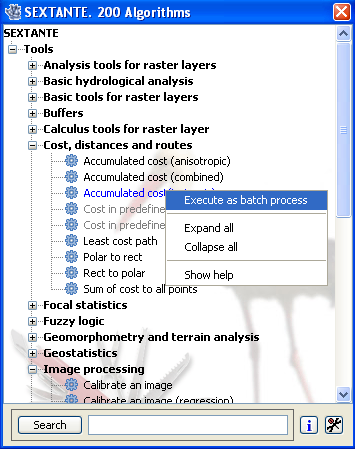
\includegraphics[width=.5\columnwidth]{batch_processing.png}
\end{center}


\section{The parameters table}

Executing a batch process is similar to performing a single execution of an algorithm. Parameter values have to be defined, but in this case we need not just a single value for each parameter, but a set of them instead, one for each time the algorithm has to be executed. Values are introduced using a table like the one shown next.

\begin{center}
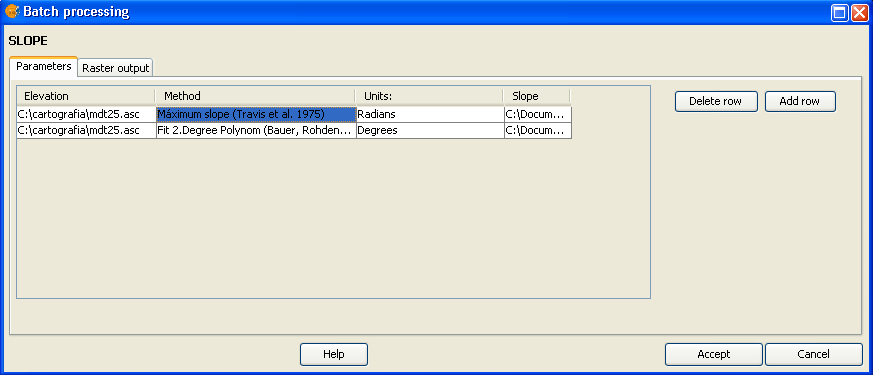
\includegraphics[width=.9\columnwidth]{batch_processing2.png}
\end{center}

Each line of this table represents a single execution of the algorithm, and each cell contains the value of one of the parameters. It is similar to the parameters tab that you see when executing an algorithm from the toolbox, but with a different arrangement.

By default, the table contains just two rows. You can add or remove rows using the buttons on the right hand side of the window.

Once the size of the table has been set, it has to be filled with the desired values

\section{Filling the parameters table}

Whatever the type of parameter it represents, every cell has a text string as its associated value. Double--clicking on a cell, this string can be edited, directly typing the desired value. For most of the parameters, however, it is more convenient to use the  button on the right hand side of the cell. Clicking on it, a dialog is shown to select the value of the parameter. The content of this dialog depends on the kind of parameter, and it features elements that make it easier to introduce the desired value. For example, for a selection parameter the list of all possible values is shown and the value can be chosen from them.


\begin{center}
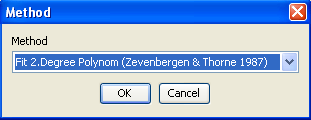
\includegraphics[width=.4\columnwidth]{batch_processing3.png}
\end{center}


For all parameter cells, if the introduced value is correct, it will be shown in black. If the value is wrong (for instance, a numerical value out of the valid range or an option that does not exists for a selecion parameter), the text will be shown in red.

\begin{center}
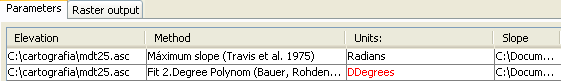
\includegraphics[width=.8\columnwidth]{batch_processing4.png}
\end{center}

The most importante different between executing an algorithm from the toolbox and executing it as part of a batch process is that input data objects are taken directly from files, and not from the set of layers already opened in the GIS. For this reason, any algorithm can be executed as a batch process even if no data objects at all are opened and the algorithm cannot be called from the toolbox.

Filenames for input data objects are introduced directly typing or, more conveniently, clicking on the button on the right hand of the cell, which shows a typical file chooser dialog. Multiple files can be selected at once. If the input parameter represents a single data object and several files are selected, each one of them will be put in a separate row, adding new ones if needed. If it represents a multiple input, all the selected files will be added to a single cell, separated by commas.

If multiple bands are required, a more complex dialog is shown, which incorporates a table for selecting both layer files and bands. Click on the cells on the left side to select the file which contains the raster layer. Then click on the left side to select the bands you want to use from that layer. To know the number of bands in a layer it would be necessary to open it. However, SEXTANTE does not open the layer, and shows instead a list of bands from 1 to 250 to select from. If you select a band that does not exist in the selected layer, an error message will be shown at execution time.

\begin{center}
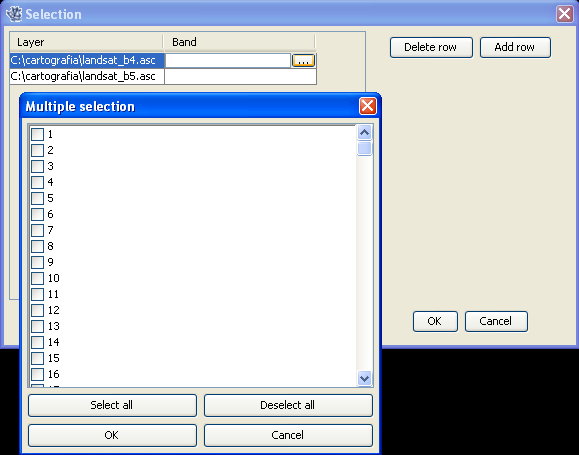
\includegraphics[width=.7\columnwidth]{batch_processing_bands.png}
\end{center}

Output data objects are always saved to a file and, unlike when executing an algorithm from the toolbox, saving to a temporary one is not permitted. You can type the name directly or use the file chooser dialog that appears when clicking on the accompanying button. This dialog differs slightly from the standard one, incorporating some additional fields for autocompletion. 
 
\begin{center}
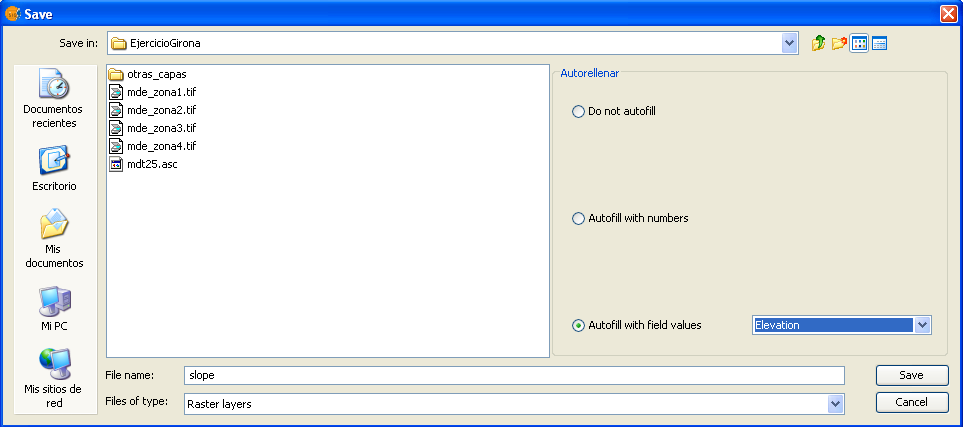
\includegraphics[width=.9\columnwidth]{batch_processing_save.png}
\end{center} 
 
If the default value (\textsf{Do not autocomplete}) is selected, SEXTANTE will just put the selected filename in the selected cell from the parameters table. If any of the other options is selected, all the cells below the selected one will be automatically filled based on a defined criteria. This way, it is much easier to fill the table, and the batch process can be defined with less effort.

Automatic filling can be done simply adding correlative numbers to the selected filepath, or appending the value of another field at the same row. This is particularly useful for naming output data object according to input ones.



\begin{center}
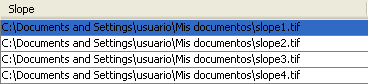
\includegraphics[width=.6\columnwidth]{batch_processing_filepath.png}
\end{center}

Cells can be selected just clicking and dragging. Selected cells can be copied and pasted in a different place of the parameters table, making it easy to fill it with repeated values.




\section{Setting the output region}

Just like when executing a single algorithm, when running a batch process you must define the extent of the region to be analyzed. The corresponding \emph{Output region} tab is similar to the one found when running a single algorithm, but only contains two options: \emph{fit to input layers} and \emph{used--defined}.

The selection will be applied to all the single executions contained in the current batch process. If you want to use different output configurations, then you must define different batch processes.

\begin{center}
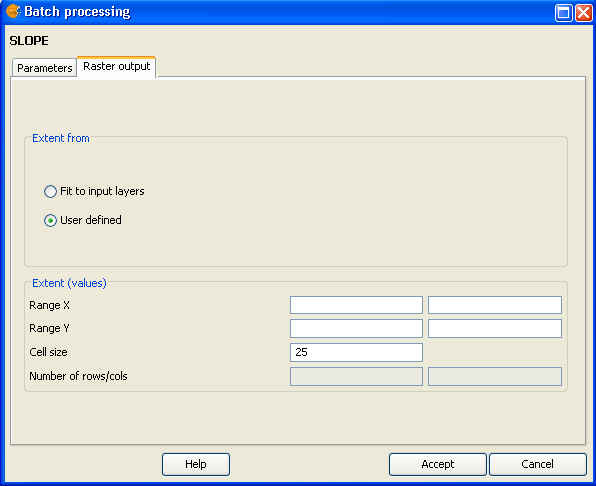
\includegraphics[width=.7\columnwidth]{batch_processing_output.png}
\end{center}

\section{Executing the batch process}

To execute the batch process once you have introduced all the necessary values, just click on \emph{OK}. SEXTANTE will show the progress of each executed algorithm, and at the end will show a dialog with information about the values used and the problems encountered during the execution of the whole process.

\begin{center}
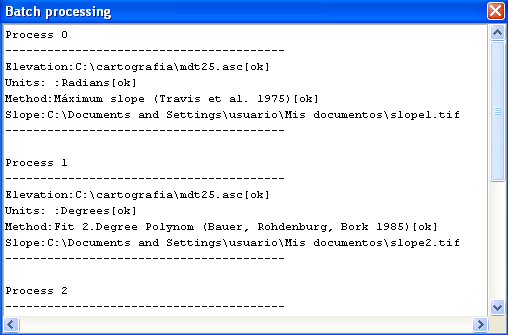
\includegraphics[width=.7\columnwidth]{batch_processing_executing.png}
\end{center}

As it happened with the iterative execution of algorithms, when executing in a batch process an algorithm that produces text output with numerical values (such as, for instance, statistics of a raster layer), its numerical outputs are presented in a table in the results manager. Each row of the table represents an execution of the algorithm, while each column contains the values of one of the numerical variables being calculated.